\chapter{Cost-sensitive logistic regression}\label{ch:7}

\begin{remark}{Outline}
In this chapter, we propose the cost-sensitive logistic regression algorithm. The model consists in 
a new logistic regression cost function, one that takes into account the real costs due to 
misclassification and correct classification. First, in Section \ref{sec:7:logistic}, we give the 
background behind logistic regression. Then, in Section \ref{sec:7:cslr}, we describe the 
cost-sensitive logistic regression. For this, we carry a deep analysis of the 
logistic regression implicit misclassification costs in Section \ref{sec:7:log_cost_analysis}. Then 
in Section \ref{sec:7:cscostfunction}, we shown a new version of the logistic regression cost 
function. 
%Afterwards, in Section \ref{sec:7:ga}, we give a brief introduction to genetic 
%algorithms, since is the model used to estimate the parameters of our proposed cost-sensitive 
%logistic regression. 
Finally, in Section \ref{sec:7:results}, we compare the results of the proposed 
algorithm against state-of-the-art methods, using the five real-world cost-sensitive databases 
presented in \partname{~\textsc{\ref{part:2}}}.
\end{remark}


\section{Logistic regression}
\label{sec:7:logistic}

Logistic regression is a classification model that, in the specific context of binary 
classification, estimates the posterior probability of the positive class, as the logistic sigmoid 
of a linear function of the feature vector \citep{Bishop2006}. The estimated probability  is 
evaluated as 
\begin{equation}
  \hat p_i = P(y=1 \vert \mathbf{x}_i) = h_{\theta}(\mathbf{x}_i) = 
  g\bigg(\sum_{j=1}^{k}{\theta^jx_i^j}\bigg),
\end{equation}
where $h_\theta(\mathbf{x}_i)$ refers to the hypothesis of $i$ given the parameters $\theta$, the 
feature vector $\mathbf{x}_i$ for example $i$ and  $g(\cdot)$ is the logistic sigmoid function 
defined as
\begin{equation}
  g(z)=\frac{1}{(1+e^{-z})} .
\end{equation}
In \figurename{~\ref{fig:ch7:1}}, the logistic sigmoid function is shown.
\begin{figure}[htbp]
  \centering
  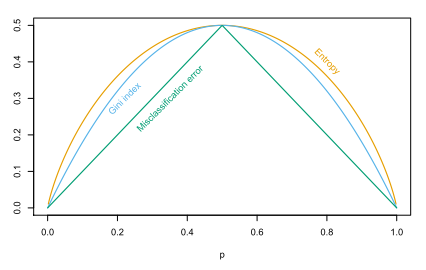
\includegraphics{ch7_fig1}
  \caption{Sigmoid function}
  \label{fig:ch7:1}
\end{figure}

The problem then becomes on finding the right parameters that minimize a given cost function.   
Usually, in the case of logistic regression, the cost function $J(\theta)$ refers to the negative   
logarithm of the likelihood, such that
\begin{equation}
  J(\theta)=\frac{1}{N}\sum_{i=1}^{N} J_i(\theta),
\end{equation}
where
\begin{align}\label{eq:7:lrcost}
  J_i(\theta) =  -y_i\log(h_\theta(\mathbf{x}_i)) -(1-y_i)\log(1-h_\theta(\mathbf{x}_i)).
\end{align}
Therefore, the parameters are estimated using the following equation
\begin{align}
  \hat \theta = \argmin_\theta J(\theta).
\end{align}

%Logistic regression estimation
There are several methods used to estimate the logistic regression, in particular, maximum 
likelihood \citep{Hastie2009}, Newton, coordinate descent \citep{Murphy2012} and dual coordinate 
descent \citep{Yu2011}. Nevertheless, all these methods rely on the assumption of convexity of the 
logistic regression cost function $J(\theta)$. In the next Appendix~\ref{ch:B} we analyze 
the convexity of the logistic regression.


\section{Cost-sensitive logistic regression}
\label{sec:7:cslr}

In this section we present our cost-sensitive logistic regression algorithm.
First, we motivate the need to modify the logistic regression, as we 
analyze the implicit costs that the logistic regression assigned to each misclassification error 
during the estimation of the parameters $\theta$. Then, we show our proposed algorithm.


\subsection{Implicit costs of the logistic regression}
\label{sec:7:log_cost_analysis}

The logistic regression cost function, as described in (\ref{eq:7:lrcost}), implicitly assume that 
false positives and false negatives have the same costs, i.e. $C_{{FP}_i} = C_{{FN}_i}$ $\forall 
i \in \{1,\cdots,N\}$. This can be easily shown by analyzing the logistic cost function for both 
values of $y_i$ and the algorithm prediction $h_\theta(\mathbf{x}_i))$:

\begin{itemize}
\item If $y_i=0$ and $h_\theta(\mathbf{x}_i) \approx 0$, then
\begin{align*}
 J_i(\theta) &= -y_i\log(h_\theta(\mathbf{x}_i)) -(1-y_i)\log(1-h_\theta(\mathbf{x}_i)) \nonumber \\
 &\approx -(0)\log((0)) -(1-(0))\log(1-(0)) \nonumber \\
 &\approx 0.
\end{align*}

\item If $y_i=0$ and $h_\theta(\mathbf{x}_i) \approx 1$, then
\begin{align*}
 J_i(\theta) &\approx -(0)\log((1)) -(1-(0))\log(1-(1)) \nonumber \\
 &\approx \infty.
\end{align*}

\item If $y_i=1$ and $h_\theta(\mathbf{x}_i) \approx 0$, then
\begin{align*}
 J_i(\theta) &\approx -(1)\log((0)) -(1-(1))\log(1-(0)) \nonumber \\
 &\approx \infty.
\end{align*}

\item If $y_i=1$ and $h_\theta(\mathbf{x}_i) \approx 1$, then
\begin{align*}
 J_i(\theta) &\approx -(1)\log((1)) -(1-(1))\log(1-(1)) \nonumber \\
 &\approx 0.
\end{align*}
\end{itemize}

\noindent Then, we collect the previous results in a cost matrix:
  \begin{table}[htbp]
    \centering
    \footnotesize
    \begin{tabular}{c|c|c}
      \multicolumn{3}{c}{}\\
      \multicolumn{1}{c|}{}  & Actual Positive& Actual Negative \\
      \multicolumn{1}{c|}{} & $y_i=1$& $y_i=0$ \\
      \hline
      Predicted Positive    & \multirow{ 2}{*}{$C_{{TP}_i}\approx 0$} & 
      \multirow{2}{*}{$C_{{FP}_i}\approx \infty$} \\
      $c_i=1$ & &\\
      \hline
      Predicted Negative    & \multirow{ 2}{*}{$C_{{FN}_i}\approx \infty$} & \multirow{ 
      2}{*}{$C_{{TN}_i}\approx 0$} \\
      $c_i=0$ & &\\
    \end{tabular}
    \caption{Logistic regression cost matrix}
    \label{tab:7:1}
  \end{table} 
  
This confirms that the logistic regression cost function implicitly assume that 
false positives and false negatives have the same costs. However, as discussed in 
Chapter~\ref{ch:4} and Chapter~\ref{ch:5}, this is not the case in several real-world 
applications.

  
\subsection{Cost-sensitive logistic regression cost function}
\label{sec:7:cscostfunction}

In order to incorporate the different real costs, as showed in 
\tablename{~\ref{tab:3:cost_matrix}}, into the logistic regression, we start by analyzing the 
expected costs that a modified logistic regression cost function should make for each 
misclassification and correct classification case.

\begin{equation*}
  J^c_i(\theta) = 
  \begin{cases}
    C_{TP_i}    & \text{if} \phantom{-}  y_i = 1 \text{ and } h_\theta(\mathbf{x}_i) \approx 1  \\
    C_{TN_i}    & \text{if} \phantom{-}  y_i = 0 \text{ and } h_\theta(\mathbf{x}_i) \approx 0  \\
    C_{FP_i}    & \text{if} \phantom{-}  y_i = 0 \text{ and } h_\theta(\mathbf{x}_i) \approx 1  \\
    C_{FN_i}    & \text{if} \phantom{-}  y_i = 1 \text{ and } h_\theta(\mathbf{x}_i) \approx 0 .
  \end{cases}
\end{equation*}

Then, as we already have the real costs, we create a new cost-sensitive logistic regression cost 
function, by including the different costs into the logistic function,

\begin{align}\label{eq:CSLR}
  J^c(\theta)=\frac{1}{N} \sum_{i=1}^{N} \bigg( y_i(h_\theta(\mathbf{x}_i) C_{TP_i} + 
  (1-h_\theta(\mathbf{x}_i))C_{FN_i})  \nonumber\\ 
  +(1-y_i)(h_\theta(\mathbf{x}_i) C_{FP_i} + (1-h_\theta(\mathbf{x}_i))C_{TN_i}) \bigg).
\end{align}

Since this  new cost function is not convex, we estimate the parameters $\theta$ with genetic 
algorithms, as this optimization heuristic does not require the underlying function to be 
differentiable or convex \citep{Haupt2004}. 

  Genetic algorithms, is an optimization technique that attempts to replicate natural evolution 
processes in which the individuals with the considered best characteristics to adapt to the 
environment are more likely to reproduce and survive. These advantageous individuals mate between 
them, producing descendants similarly characterized, so favorable characteristics are preserved and 
unfavorable ones destroyed, leading to the progressive evolution of the species. The model aims 
to improve the solution to a problem by keeping the best combination of input variables 
\citep{Haupt2004}. 

\section{Experiments}
\label{sec:7:results}

\begin{table}[b]
    \centering
    \footnotesize
    \begin{tabular}{l l r@{\hskip 0in}c@{\hskip 0in}l r@{\hskip 0in}c@{\hskip 0in}l r@{\hskip 
    0in}c@{\hskip 0in}l  } %sum 7.7
    \hline
    \bf{Family} & \bf{Algorithm} & \multicolumn{3}{c}{\bf{Fraud}} & 
    \multicolumn{3}{c}{\bf{Churn}} & \multicolumn{3}{c}{\bf{Credit 1}} \\ 
    \hline
CI&LR-t & 0.0092 &$\pm$& 0.0002 & -0.0001 &$\pm$& 0.0002 & 0.0177 &$\pm$& 0.0126\\ 
&LR-u & 0.1243 &$\pm$& 0.0387 & 0.0039 &$\pm$& 0.0492 & 0.4118 &$\pm$& 0.0313\\ 
\hline 
CPS&LR-r & 0.3077 &$\pm$& 0.0301 & 0.0484 &$\pm$& 0.0375 & 0.3965 &$\pm$& 0.0263\\ 
&LR-o & 0.2793 &$\pm$& 0.0185 & 0.0316 &$\pm$& 0.0228 & 0.3301 &$\pm$& 0.0109\\ 
\hline 
BMR&LR-t-BMR & 0.4552 &$\pm$& 0.0203 & 0.1082 &$\pm$& 0.0316 & 0.2189 &$\pm$& 0.0541\\ 
\hline 
CST&CSLR-t & \bf{0.6113} &\bf{$\pm$}& \bf{0.0262} & \bf{0.1118} &\bf{$\pm$}& \bf{0.0484} & 
\bf{0.4554} &\bf{$\pm$}& \bf{0.1039}\\ 
\hline
  \multicolumn{11}{c}{(Models with the highest savings are marked in bold)}
  \end{tabular}
    \caption{Results of the algorithms measured by savings}
    \label{tab:7:results_savings}
  \end{table}
\begin{table}
    \centering
    \footnotesize
    \begin{tabular}{l l r@{\hskip 0in}c@{\hskip 0in}l r@{\hskip 0in}c@{\hskip 0in}l  } %sum 7.7
    \hline
    \bf{Family} & \bf{Algorithm} &  \multicolumn{3}{c}{\bf{Credit 2}} 
& \multicolumn{3}{c}{\bf{Marketing}} \\ 
    \hline
CI&LR-t & 0.0039 &$\pm$& 0.0012 & -0.2931 &$\pm$& 0.0602\\ 
&LR-u & 0.1850 &$\pm$& 0.0231 & 0.2200 &$\pm$& 0.0376\\ 
\hline 
CPS&LR-r & 0.2650 &$\pm$& 0.0115 & 0.4210 &$\pm$& 0.0267\\ 
&LR-o & 0.2554 &$\pm$& 0.0090 & 0.3129 &$\pm$& 0.0277\\ 
\hline 
BMR&LR-t-BMR & \bf{0.3148} &\bf{$\pm$}& \bf{0.0094} & \bf{0.4973} &\bf{$\pm$}& \bf{0.0084}\\ 
\hline 
CST&CSLR-t & 0.2748 &$\pm$& 0.0069 & 0.4484 &$\pm$& 0.0072\\ 
\hline 
  \multicolumn{8}{c}{(Models with the highest savings are marked in bold)}
  \end{tabular}
    \caption{Continuation of \tablename{~\ref{tab:7:results_savings}}.}
    \label{tab:7:results_savings2}
  \end{table}

For the experiments we use five datasets from four different real world example-dependent 
cost-sensitive problems: Credit card fraud detection (see Section~\ref{sec:4:fraud}), credit 
scoring (see Section~\ref{sec:4:creditscoring}), churn modeling (see Section~\ref{sec:5:churn}) and 
direct marketing (see Section~\ref{sec:5:directmarketing}). The different datasets are summarized 
in \tablename{~\ref{tab:6:databases}}.

In particular, we are interested in comparing the results of the different logistic regression 
models. First we train a logisitc regression ($LR$) using the training ($t$), under-sampled 
($u$), cost-proportionate rejection-sampling  ($r$) \citep{Zadrozny2003}  and  cost-proportionate 
over-sampling ($o$) \citep{Elkan2001} datasets. Afterwards,  we evaluate the results of  the 
algorithms using $BMR$, see Chapter~\ref{ch:6}. Lastly, we calculate the cost-sensitive 
logistic  regression ($CSLR$). We use the logistic regression implementation of
\textit{Scikit-learn} \citep{Pedregosa2011}, and the \textit{CostCla} library, see 
Appendix~\ref{ch:A}, for the cost-sensitive algorithms. Unless otherwise stated, the random 
selection of the training set was repeated 50 times, and in each time the models were trained and 
results collected, this allows us to measure the stability of the results.
  
In \tablename{~\ref{tab:7:results_savings}}, we show the results of each algorithm in the different 
databases measured by savings. Firstly, the proposed $CSLR$ has the highest savings in the 
fraud, churn and credit 1 databases, moreover, in the credit 2 and marketing databases, it 
is the second best model. It is interesting to see how different the results from a standard 
logistic regression and the cost-sensitive logistic 
regression are. Moreover, we also calculate the results of the $F_1Score$ for each model, as 
shown in \tablename{~\ref{tab:7:results_fscore}}. It is observed that the $CSLR$ algorithm is not 
the one that gives the best results measured by $F_1Score$. In fact, there is not a clear relation 
between the results measured by savings or  $F_1Score$.

\begin{table}
    \centering
    \footnotesize
    \begin{tabular}{l l r@{\hskip 0in}c@{\hskip 0in}l r@{\hskip 0in}c@{\hskip 0in}l r@{\hskip 
    0in}c@{\hskip 0in}l  } %sum 7.7
    \hline
    \bf{Family} & \bf{Algorithm} & \multicolumn{3}{c}{\bf{Fraud}} & 
    \multicolumn{3}{c}{\bf{Churn}} & \multicolumn{3}{c}{\bf{Credit 1}} \\ 
    \hline
CI&LR-t & 0.1531 &$\pm$& 0.0045 & 0.0000 &$\pm$& 0.0000 & 0.0494 &$\pm$& 0.0277\\ 
&LR-u & 0.0241 &$\pm$& 0.0163 & 0.1222 &$\pm$& 0.0098 & 0.3160 &$\pm$& 0.0314\\ 
\hline 
CPS&LR-r & 0.1846 &$\pm$& 0.0123 & 0.1258 &$\pm$& 0.0111 & 0.3597 &$\pm$& 0.0156\\ 
&LR-o & 0.1776 &$\pm$& 0.0117 & 0.1085 &$\pm$& 0.0203 & \bf{0.3769} &\bf{$\pm$}& \bf{0.0067}\\ 
\hline 
BMR&LR-t-BMR & 0.1384 &$\pm$& 0.0044 & \bf{0.1370} &\bf{$\pm$}& \bf{0.0150} & 0.1915 &$\pm$& 
0.0340\\ 
\hline 
CST&CSLR-t & \bf{0.2031} &\bf{$\pm$}& \bf{0.0065} & 0.1134 &$\pm$& 0.0151 & 0.1454 &$\pm$& 0.0517\\ 
\hline
  \multicolumn{11}{c}{(Models with the highest $F_1Score$ are marked in bold)}
  \end{tabular}
    \caption{Results of the algorithms measured by $F_1Score$}
    \label{tab:7:results_fscore}
  \end{table}
  
\begin{table}
    \centering
    \footnotesize
    \begin{tabular}{l l r@{\hskip 0in}c@{\hskip 0in}l r@{\hskip 0in}c@{\hskip 0in}l  } %sum 7.7
    \hline
    \bf{Family} & \bf{Algorithm} &  \multicolumn{3}{c}{\bf{Credit 2}} 
& \multicolumn{3}{c}{\bf{Marketing}} \\ 
    \hline
CI&LR-t & 0.0155 &$\pm$& 0.0037 & 0.2702 &$\pm$& 0.0125\\ 
&LR-u & \bf{0.3890} &\bf{$\pm$}& \bf{0.0053} & 0.3440 &$\pm$& 0.0083\\ 
\hline 
CPS&LR-r & 0.3793 &$\pm$& 0.0049 & 0.3374 &$\pm$& 0.0101\\ 
&LR-o & 0.3804 &$\pm$& 0.0044 & \bf{0.3568} &\bf{$\pm$}& \bf{0.0102}\\ 
\hline 
BMR&LR-t-BMR & 0.3572 &$\pm$& 0.0045 & 0.2954 &$\pm$& 0.0079\\ 
\hline 
CST&CSLR-t & 0.3363 &$\pm$& 0.0045 & 0.2339 &$\pm$& 0.0051\\ 
\hline 
  \multicolumn{8}{c}{(Models with the highest $F_1Score$ are marked in bold)}
  \end{tabular}
    \caption{Continuation of \tablename{~\ref{tab:7:results_fscore}}.}
    \label{tab:7:results_fscore2}
  \end{table}
  
Finally, we compute the perBest statistic  for the savings and the $F_1Score$. This statistic is 
calculated as the average result of each algorithm compared with the best in each set. The results 
are shown in \figurename{~\ref{fig:7:comparison_per_best}}. On average, the $CSLR$ is the best 
model, as it yield to 95.5\% of the best model in the different databases. Nevertheless, when 
measured by $F_1Score$, it only yield to 74.7\% of the best model. This leads to the conclusion 
of the importance of using a cost-sensitive measure such as savings when evaluating real-world 
example-dependent cost-sensitive problems. 

\begin{figure} 
  \centering
  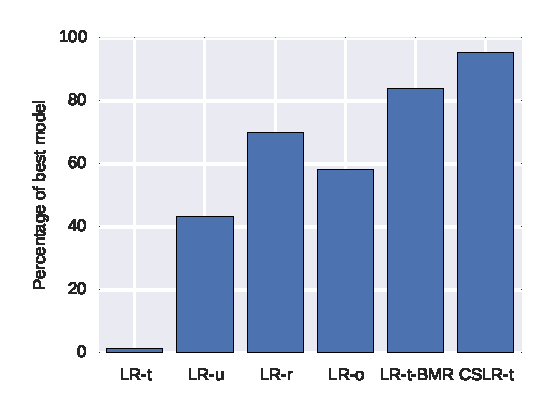
\includegraphics{ch7_fig3}
  \caption{\textbf{Comparison of the average savings and $F_1Score$ of the algorithms versus the 
    the best model.} The models that perform the best measured by $F_1Score$ are not the best 
  in terms of savings.}
  \label{fig:7:comparison_per_best}
\end{figure}

Moreover, it is observed that the standard logistic regression trained using the training set is 
the model that performs the worst measured by both savings and $F_1Score$. This is related not only 
to the cost-sensitivity of the problems, but also to the highly unbalanced distribution of positive 
and negatives presented in all the databases. This is the reason why by using an under-sampling 
procedure, the results are improved by both measures.